\section{Останній розділ}

Використовуючи методи математичної лінгвістики, тобто тієї галузі лінгвістики,
що займається вивченням структури природних мов, для виведення та встановлення
певних правил та мовних законів

\subsection{Корпус української мови}
\subsection{Корпус іспанської мови}
\subsection{Порівняння}


\begin{figure}[ht]
  \begin{center}
    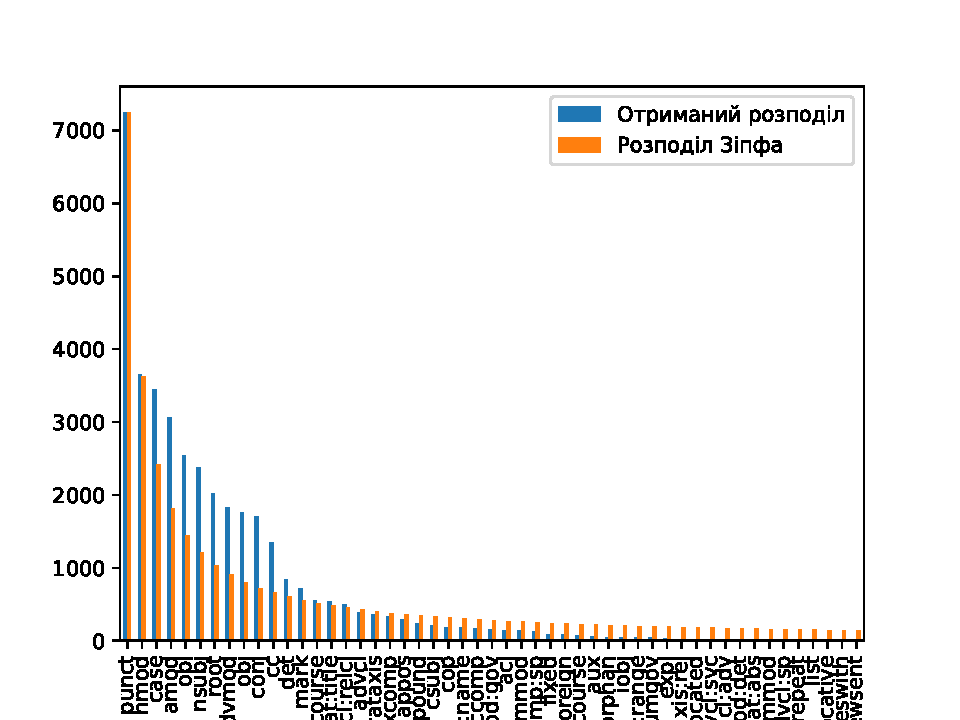
\includegraphics[width=\linewidth]{chart_uk_deprel.pdf}
  \end{center}
  \caption{Зберігання даних у вигляді знімків станів}
  \label{img:0}
\end{figure}

\begin{figure}[ht]
  \begin{center}
    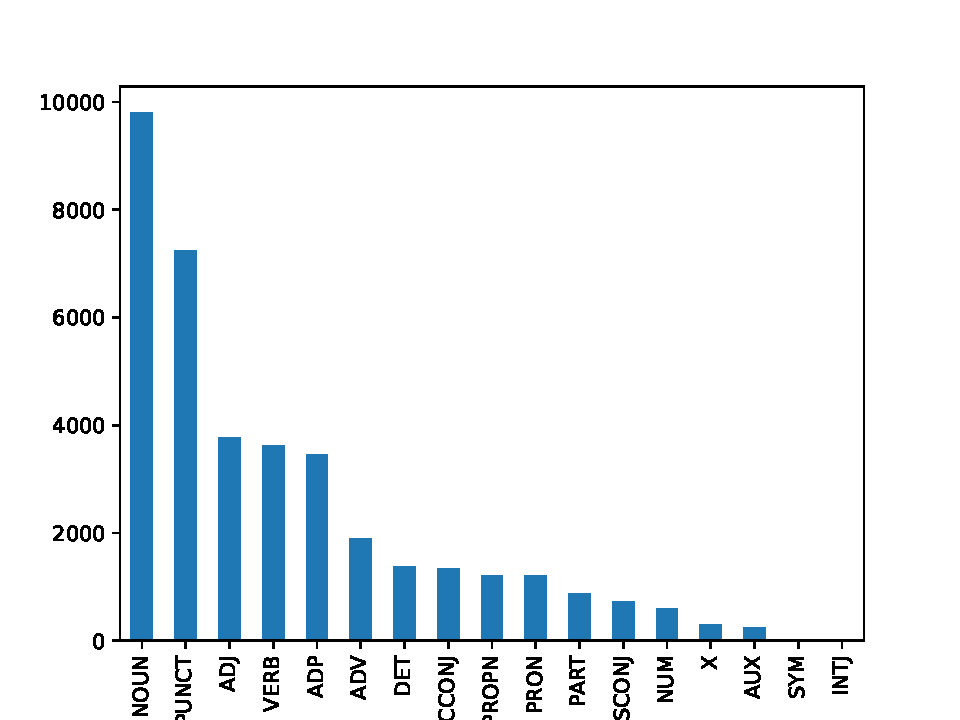
\includegraphics[width=\linewidth]{chart_uk_upos.pdf}
  \end{center}
  \caption{Зберігання даних у вигляді знімків станів}
  \label{img:1}
\end{figure}

\begin{figure}[ht]
  \begin{center}
    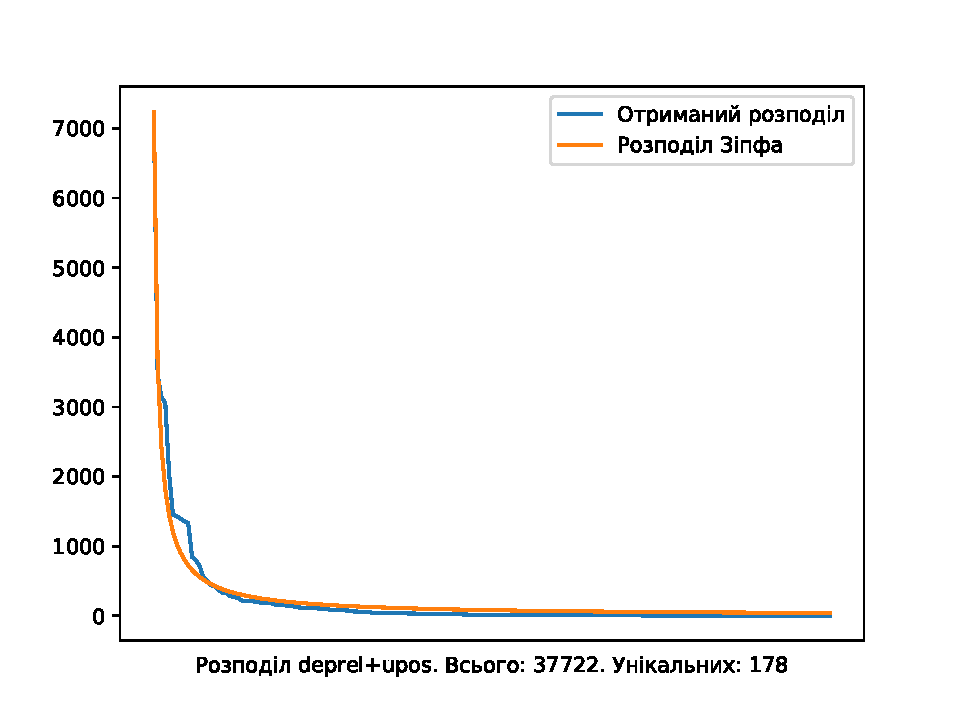
\includegraphics[width=\linewidth]{chart_uk_deprel_upos.pdf}
  \end{center}
  \caption{Зберігання даних у вигляді знімків станів}
  \label{img:2}
\end{figure}

\begin{figure}[ht]
  \begin{center}
    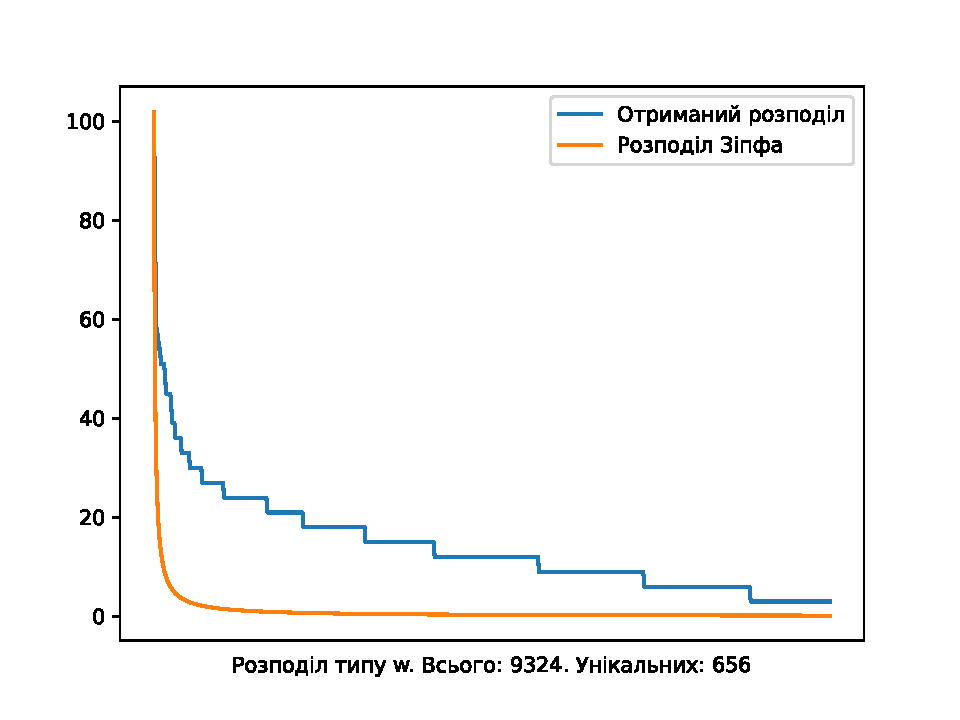
\includegraphics[width=\linewidth]{chart_uk_type_w.pdf}
  \end{center}
  \caption{Зберігання даних у вигляді знімків станів}
  \label{img:3}
\end{figure}

\begin{figure}[ht]
  \begin{center}
    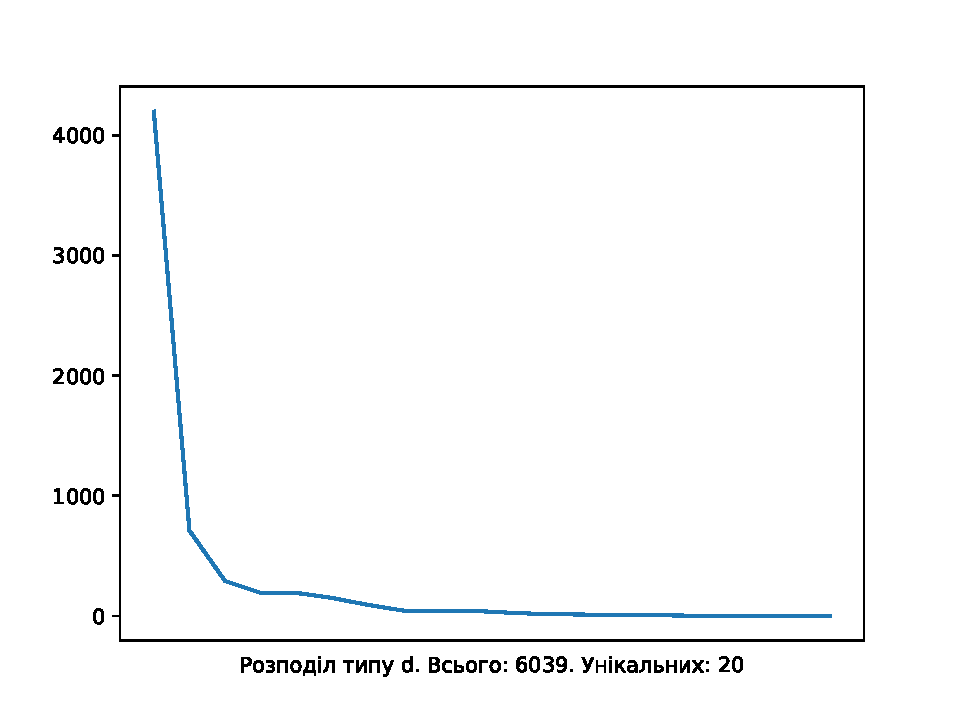
\includegraphics[width=\linewidth]{chart_uk_type_d.pdf}
  \end{center}
  \caption{Зберігання даних у вигляді знімків станів}
  \label{img:4}
\end{figure}

\begin{figure}[ht]
  \begin{center}
    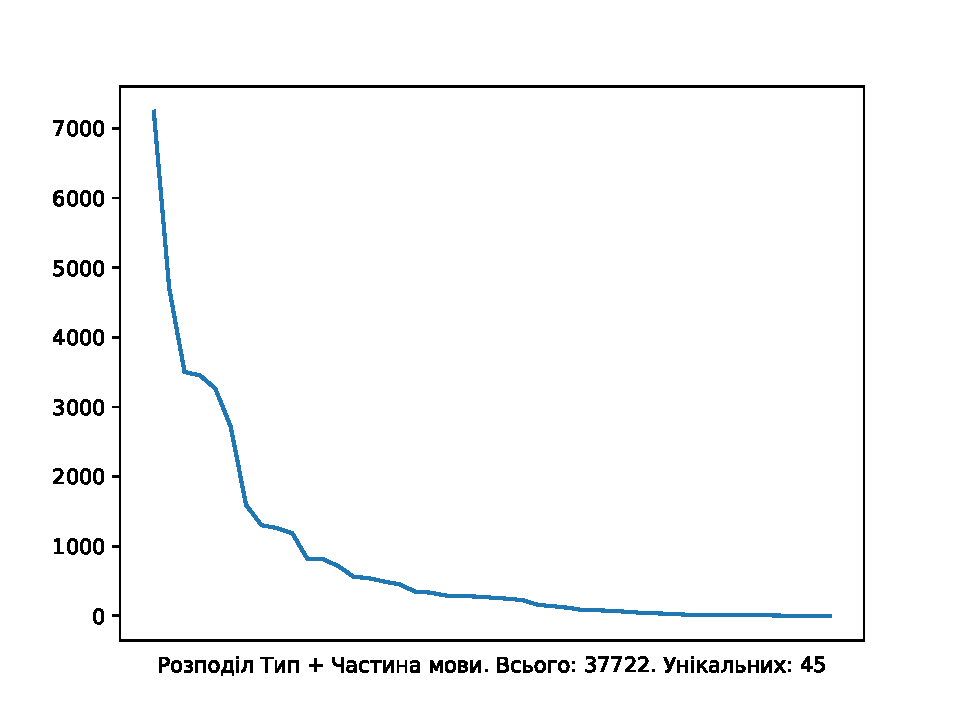
\includegraphics[width=\linewidth]{chart_uk_type_upos.pdf}
  \end{center}
  \caption{Зберігання даних у вигляді знімків станів}
  \label{img:5}
\end{figure}

\begin{figure}[ht]
  \begin{center}
    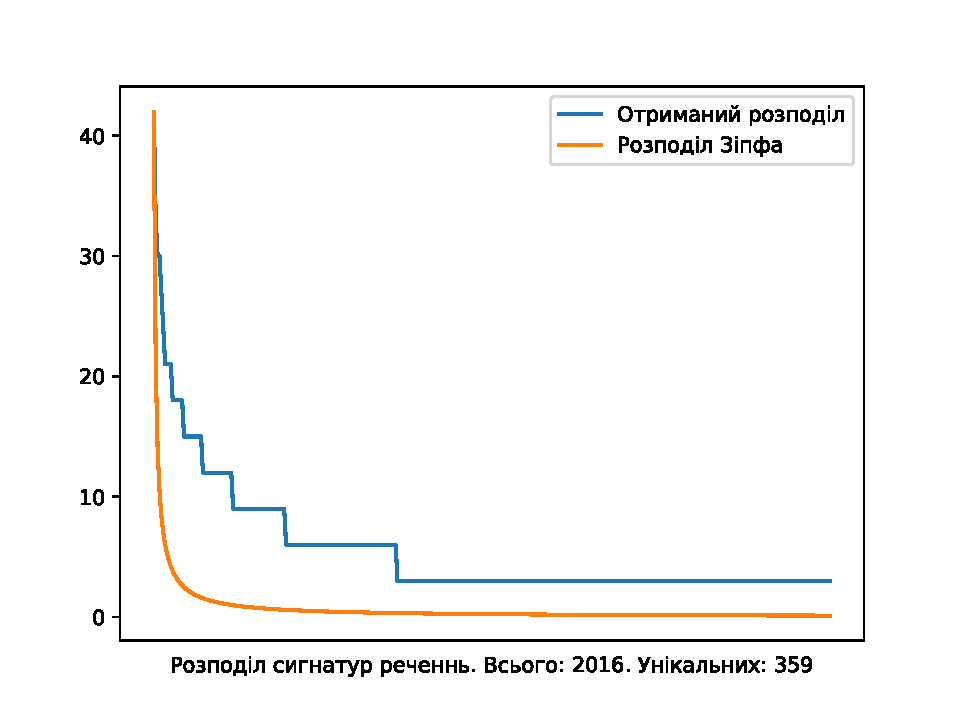
\includegraphics[width=\linewidth]{article/images/chart_uk_sent_d_w_n.pdf}
  \end{center}
  \caption{Зберігання даних у вигляді знімків станів}
  \label{img:6}
\end{figure}